\subsection{Part A}
\subsubsection{Objectives}

\begin{itemize}
    \item 熟悉 xv6 虚拟内存系统
    \item 给 xv6 添加一些现代操作系统常有的功能
\end{itemize}

\subsubsection{Steps}

\begin{enumerate}
    \item 找到原始 xv6 和 Linux 系统在访问空指针的区别
    \item 理解 xv6 如何建立页表 (page table),并且改动使其将前两页忽略 (unmapped)
    \item 改进 xv6 使其能在访问空指针的时候使用 trap 并且 kill 掉进程
\end{enumerate}

首先设置 qemu 的路径(我的安装在 root 用户下,但是实际使用另一个账户运行,所以运行指令为 `sudo make qemu-nox`)
\begin{textcode}
# If the makefile can't find QEMU, specify its path here
QEMU := /root/install/qemu-6.828-2.9.0/i386-softmmu/qemu-system-i386
\end{textcode}

编写一个程序,访问空指针,原代码见 \textbf{./xv6 VM Layout/user/nulldereference.c}

\begin{ccode}
#include "types.h"
#include "stat.h"
#include "user.h"

int main(int argc, char const *argv[])
{
    char *a;
    printf(1, "%d\n", *a);
    exit();
}
\end{ccode}

修改 \textbf{./xv6 VM Layout/user/makefile.mk},添加我们编写的新程序

\begin{bashcode}
# user programs
USER_PROGS := \
    cat\
    echo\
    forktest\
    grep\
    init\
    kill\
    ln\
    ls\
    mkdir\
    rm\
    sh\
    stressfs\
    tester\
    usertests\
    wc\
    zombie\
    nulldereference # new program we add
\end{bashcode}

结果如下,发现指针 `a` 指向未知的一串值

\begin{textcode}
xv6...
lapicinit: 1 0xfee00000
cpu1: starting
cpu0: starting
init: starting sh
$ nulldereference
-115
$ 
\end{textcode}

当我们在 \textbf{Linux} 中运行类似的程序

\begin{textcode}
zt@iZuf60n9722bkqxpt1w1sgZ:~/ECNU-OSLab/lab4/test$ ./main
Segmentation fault
\end{textcode}

\subsubsection{page tabe}

32 位无符号地址被分为三个部分,第一个部分为 page directory index,第二部分为 page table index,第三部分表示 offset with page。这样每个页表构成 $2^{10}$ 个页表项,每个页表项有 $2^{12}$ 字节。然后我们也可以通过简单的位运算获取线性地址的这些部分。

回顾一下 x86 系统中使用两级树结构存放内存,每一级都是一个 1024 项的表,每一项是一个 32 位的数据,一般来说前 20 位表示物理地址的前 20 位,也就是我们要做的映射结果;后 12 位表示各种 flag。第一级存了1024个 page table,我们把这一级称为 page directory。因为每个 page table 正好有 \textbf{1024x4=4096} 大,前 20 位刚好可以表示一个 page table 的头,所以这里第一级的结构里面放的都是页表。第二级存放了 1024 项 physical page number(PPN) 这 20 位替换虚拟地址中的前二十位就是物理地址了。总的来说,虚拟地址替换为物理地址的步骤时,前 10 位在 page directory 中找到 page table,然后 10 位找到 PPN,最后替换虚拟地址的前 20 位。原理如下图 \ref{fig:1} 所示

\begin{figure}[h]
    \centering
    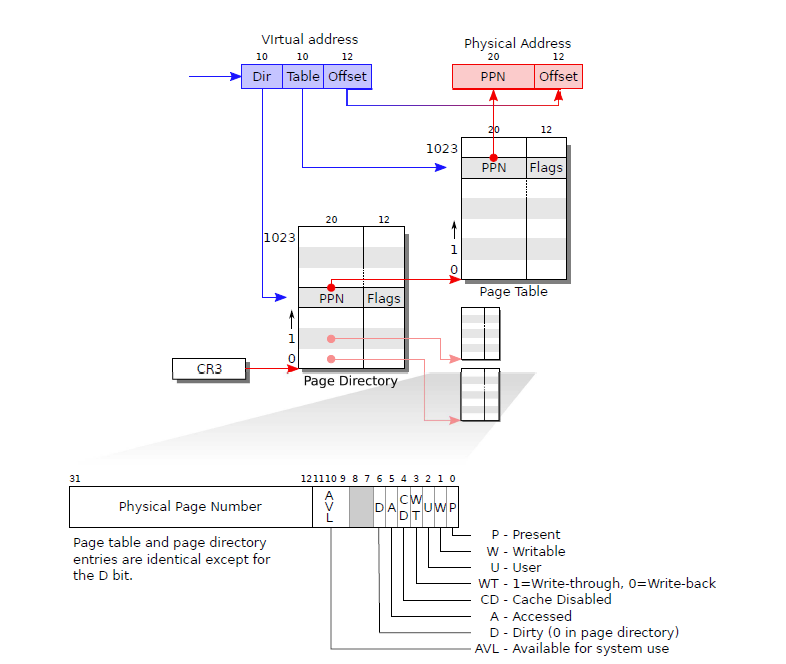
\includegraphics[width=0.8\textwidth]{img/pagemodel.PNG}
    \caption{xv6 page model}
    \label{fig:1}
\end{figure}

\textbf{./xv6 VM Layout/kernel/mmu.h}

\begin{ccode}
// A linear address 'la' has a three-part structure as follows:
//
// +--------10------+-------10-------+---------12----------+
// | Page Directory |   Page Table   | Offset within Page  |
// |      Index     |      Index     |                     |
// +----------------+----------------+---------------------+
//  \--- PDX(la) --/ \--- PTX(la) --/

// page directory index
#define PDX(la)		(((uint)(la) >> PDXSHIFT) & 0x3FF)

// page table index
#define PTX(la)		(((uint)(la) >> PTXSHIFT) & 0x3FF)

// construct linear address from indexes and offset
#define PGADDR(d, t, o)	((uint)((d) << PDXSHIFT | (t) << PTXSHIFT | (o)))
\end{ccode}

每个页表项需要一些 flag 设置他们的属性,比如说 Writeable 表示可以写入,Present 表示这个页表已经被用到了。还可以指定被当成缓存时的各种策略

\textbf{./xv6 VM Layout/kernel/mmu.h}

\begin{ccode}
// Page table/directory entry flags.
#define PTE_P		0x001	// Present
#define PTE_W		0x002	// Writeable
#define PTE_U		0x004	// User
#define PTE_PWT		0x008	// Write-Through
#define PTE_PCD		0x010	// Cache-Disable
#define PTE_A		0x020	// Accessed
#define PTE_D		0x040	// Dirty
#define PTE_PS		0x080	// Page Size
#define PTE_MBZ		0x180	// Bits must be zero
\end{ccode}

\subsubsection{memory layout}

\begin{figure}[h]
    \centering
    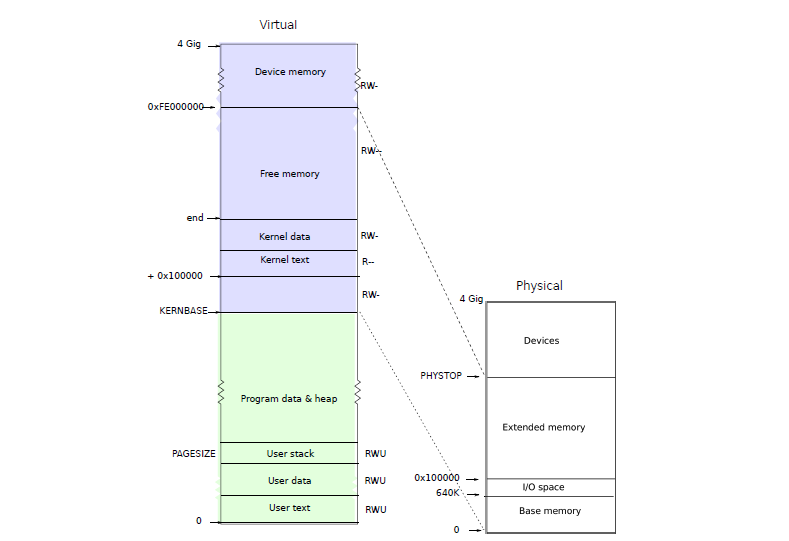
\includegraphics[width=0.8\textwidth]{img/memlayout.PNG}
    \caption{xv6 memory layout}
    \label{fig:2}
\end{figure}

用户内存从 0 开始一直到 KERNBASE。在 \textbf{./xv6 VM Layout/include/types.h} 中我们看到 NULL 被定义为 0。因此一个空指针会访问到 User text 部分,这部分的页表 flag 上有 \textbf{Present} 因此会被认为是一个合法的内存访问。现在我们希望把前两页空出来,这样当前两页将没有 `Present` flag,访问的时候 kernel 就会帮我们处理错误。

于是我们的任务主要就是:使得程序 (User text) 从 0x2000 开始存放,留出两页的空间,涉及到的更改有:

\begin{itemize}
    \item exec 执行程序会涉及到程序装载
    \item fork 复制出新的进程涉及到内存复制(程序装载)
    \item userinit 装载第一个用户程序需要特殊操作(涉及修改makefile)
    \item 修改相应的用户传入的地址的检查
\end{itemize}


\subsubsection{Code: exec}

exec 函数首先会检查 page table directory 是否设置,以及检查 elf header。不过我们的主要关注它如何分配内存

让我们先理解一些函数(无关紧要的细节已经被忽略)

\begin{itemize}
    \item \textbf{./xv6 VM Layout/kernel/kalloc.c kalloc} 该函数分配一个 4096 长度的物理内存空间
    \item \textbf{./xv6 VM Layout/kernel/vm.c walkpgdir} 返回页表地址
    \item \textbf{./xv6 Vm Layout/kernel/vm.c allocuvm} 为某个进程的页表分配新的空间,从 oldsz 增长到 newsz
    \item \textbf{./xv6 VM Layout/kernel/vm.c mappages} 该函数把会根据新分配的物理空间(4096长度)建立页表。也就是说会建立参数 la (虚拟地址) 到 pa (物理地址) 之间的映射。我们可以看到获取 `la` 的地址后会检查是否该地址已经被其他物理地址占用了(\textbf{panic("remap")}),否则就把 flag 加上 Present 一起添加。由之前的定义,相邻 page table directory 本来就有相邻的地址,如果这个 page table 满了自动就会应用到下一个 page table 中。(其实也可以看作是 $2^{20}$ 个连续页表)
\end{itemize}







